%\documentclass[draft]{article}

\documentclass{article}

\usepackage{scrextend}
\changefontsizes[7.1pt]{7.1pt}

\usepackage[utf8]{inputenc}
\usepackage[german]{babel}

\setlength{\footskip}{15pt}%Set footer dist.

\usepackage{chemfig}
\usepackage{graphicx}
\graphicspath{ {img/} }
\usepackage{hyperref}
\usepackage{multicol}
\usepackage{amsmath}
\usepackage{fancyvrb}

\usepackage{parskip}%no paragraph indents
\usepackage[landscape, margin=1cm]{geometry}
%\usepackage{adjustbox}

\begin{document}

\begin{multicols*}{3}
%\setlength{\columnseprule}{0.4pt}


\title{Physik}
\author{Gian Hiltbrunner}
\maketitle

\section{Grundlegende Konzepte der Naturwissenschaften}
  \subsection{Einheiten}

  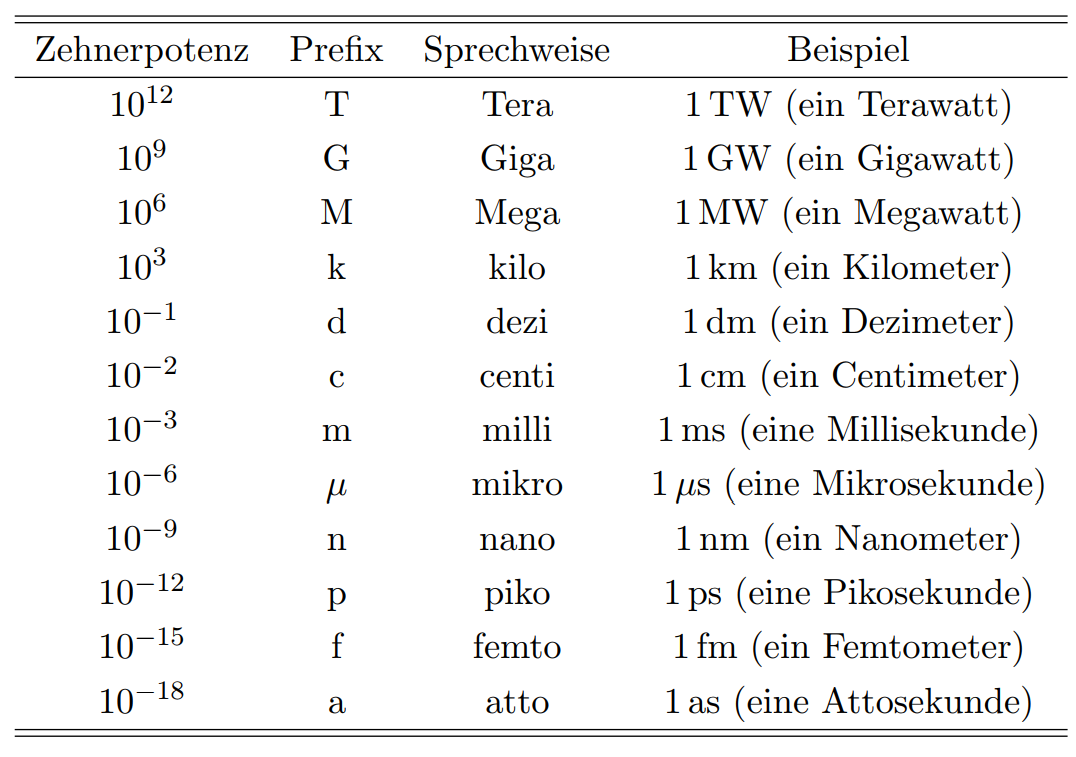
\includegraphics[scale=0.22, angle=0]{units}

  \textbf{Quadratische und kubische Einheiten ebenfalls potenzieren!}

  \subsection{Geometrie}
    $$\sin(\alpha) = \frac{G}{H};
    \cos(\alpha) = \frac{A}{H};
    \tan{\alpha} = \frac{G}{A}$$

    $$\cos ^2{x}+\sin ^2{x} = 1$$
    Kugel
    $$V=\frac{4}{3}\pi r ^3, A= 4\pi r^2$$

    Kreuzprodukt
    $$u\times v={\begin{pmatrix}s_{1}\\s_{2}\\s_{3}\end{pmatrix}}={\begin{pmatrix}u_{2}v_{3}-u_{3}v_{2}\\u_{3}v_{1}-u_{1}v_{3}\\u_{1}v_{2}-u_{2}v_{1}\end{pmatrix}}$$

  \subsection{Konstanten und Anderes}
  Avogadro: $N_A=6.022 \times 10^{23} mol^{-1}$\\
  Volumen: $1 m^3 = 1000 L$
  \\$[°C] = [K] - 273.15$
\section{Mechanik}
  \subsection{Bewegung in einer Dimension}
  $$v = \frac{\Delta x}{\Delta t}$$
  \subsubsection{Momentane Geschwindigkeit}
  $${\displaystyle {\vec {v}}={\underset {\Delta t\rightarrow 0}{\lim }}{\frac {\Delta {\vec {r}}}{\Delta t}}={\frac {\mathrm {d} {\vec {r}}}{\mathrm {d} t}}={\dot {\vec {r}}}}$$
  $$x(t) - x(0) = \int_{0}^{t} v(t')dt'$$
  \subsection{Momentane Beschleunigung}
  $${\vec {a}}(t)={\frac {\mathrm {d} {\vec {v}}(t)}{\mathrm {d} t}}={\dot {\vec {v}}}(t)$$
  $$v(t) - v(0) = \int_{0}^{t} a(t')dt' + [v_0]$$

  \subsection{Kreisbewegung}
  $$\omega ={\frac {d\varphi }{dt}}, {\displaystyle \omega ={\frac {2\pi }{T}}};\omega = 2\pi f$$
  Zentripetalbeschleunigung
  $$a_{{{\mathrm  {Z}}}}={\frac  {v^{2}}{r}}=\omega ^{2}r$$
  $$\mathrm {v} _{\perp }={\frac {d\phi }{dt}}\,r=\omega \cdot r$$
  \subsection{Trägheit (1. Newton)}
  Ein Körper verharrt im Zustand der Ruhe oder der gleichförmig geradlinigen Bewegung,
  sofern er nicht durch einwirkende Kräfte zur Anderung seines Zustands gezwungen wird.

  \subsection{Bewegungsgleichung (2.Newton)}
  $$m\vec{a} = \frac{d(m\vec{v})}{dt} = \frac{d\vec{p}}{dt} = \vec{F}(t,\vec{r},\vec{v})$$
  z.B.: Bei Auslenkung $x(t)\rightarrow \frac{d^2x(t)}{dt^2}$
  \\$[F] = kg*m/s^2$
  \subsection{3. Newton}
  $$actio = reactio$$

  \subsection{Hooksches Gesetz}
  $$F = k(l - l_0)$$

  \subsection{Superpositionsprinzip der Kräfte}
  $$\vec{F}_K = \vec{F}_1 + \vec{F}_2 + ... + \vec{F}_n = \sum_{i=1}^{n} \vec{F}_i$$
  "Die Gesamtkraft auf einen Körper ist die Summe der einzelnen Kräfte, die auf
  ihn wirken."

  \subsection{Impuls}
  $$\vec{p} = m\vec{v}; \Delta p = F\Delta t  \quad [p] = Ns$$

  \subsection{Reaktionsprinzip}

  \textbf{'Actio = Reactio'}

  $$\vec{F}_{Hin} = -\vec{F}_{Rück}$$

  \subsection{Harmonische\\ Schwingungsgleichung}
  $$\ddot{z}=-\omega ^2 z,\omega_0=\sqrt{\frac{k}{m}}$$

  $$y(t)=y_0\cdot\sin(2\pi f t+\varphi_0), f = {1 \over T}$$

  wobei $y_0$ = Amplitude, $\varphi_0$ = Nullphasenwinkel\\

  $$T = 2\pi\theta =2\pi {\sqrt {\frac {m}{k}}}.$$
  $$f = \frac{1}{T} = {\frac {1}{2\pi }}{\sqrt {\frac {k}{m}}}$$

  \subsection{Gedämpfte Schwingung}
  $$m\frac{d^2x}{dt^2} = -kx - \gamma\frac{dx}{dt}$$

  Lösung der Diff.gleichung:
  $$x(t) = Ae^{\frac{-t}{2r}}\sin[\sqrt{1-(\frac{r}{2})^2}\frac{t}{\theta}+\delta]$$

  \subsection{Zentrifugalkraft}

  $$\vec{F}_{ZF} = m r_0\omega ^2 \begin{pmatrix} \cos(\phi(t)) \\ \sin(\phi(t)) \\ 0 \end{pmatrix} = m\omega ^2\vec{r}$$

  \subsection{Newtonsches Gravitationsgesetz}
  $$F_G= G\frac{m_1m_2}{r^2}$$
  $G = 6.674 * 10 ^{-11} \frac{Nm^2}{kg^2}$

  \subsection{Erdanziehung}
  $$F_E = mg$$

  \subsection{Coulombsches Gesetz}
  $$F_C = \frac{|q_1q_2|}{4\pi\epsilon _0 r^2}$$
  $\epsilon _0= 8.854 * 10^{-12} \frac{C^2}{Nm^2}, e=1{,}602\,176\cdot 10^{-19}\ \mathrm {C}$

  \subsection{Hooksches Gesetz}
  $$F = -k(l-l_0); k=\frac{EA}{L_0}$$

  \subsection{Hooksches Gesetz für makro. Körper}
  $$\sigma = -E\epsilon$$

  \subsection{Kinetische Energie}
  $$E_{kin}(t)= \frac{1}{2}m \vec{v}^2 = \frac{p^2}{2m}$$

  \subsection{Arbeit}
  $$W_C=\int_{C}\vec{F}\bullet d\vec{r}$$
  $${\displaystyle W={\vec {F}}\cdot {\vec {s}}=|{\vec {F}}|\,|{\vec {s}}|\,\cos \langle \left({\vec {F}},{\vec {s}}\right)\,}$$

  \subsection{Leistung}
  $$P = \frac{dW}{dt} = \vec{F} \bullet \vec{v}$$

  \subsection{Arbeit als Integral der Leistung}
  $$\Delta W = \int_{t_0}^{t_1} \vec{F}(t) \bullet \vec{v}(t) dt = \int_{t_0}^{t_1} P(t) dt$$

  \subsection{Konservative Kraft}
  ‘Eine Kraft ist konservativ, wenn die Gesamtarbeit, die sie an einem Körper
  verrichtet, der sich auf einer beliebigen geschlossenen Bahn bewegt, Null
  ist.’
  \subsection{Potentielle Energie}

  $$\Delta E_{pot} = \int_{C} \vec{F}_K \bullet d\vec{r} = -W_C$$
  Im Schwerefeld der Erde:
  $$E_{pot}=mgh$$
  $g_{Erde} = 9.81 \frac{m}{s^2}$

  \subsection{Kraft aus Potentieller Energie}
  $$F_K = - \frac{dE_{pot}}{dx} = - \frac{dV}{dx}$$

  \subsection{Hamiltonian}

  $$\mathcal{H}(\vec{p}_1,...,\vec{p}_n, \vec{r}_1,...,\vec{r}_n) = \sum_{i=1}^{n} \frac{\vec{p}_i^2}{2m_i} + \frac{1}{2} \sum_{i,j =1; i \neq j}^{n} V(\vec{r}_i, \vec{r}_j)$$

  \subsection{Zustand von Vielteilchensystemen}

  Daher nennt man in der Mechanik von Vielteilchensystemen den Satz von Vektoren
  $(\vec{p}_1,...,\vec{p}_n, \vec{r}_1,...,\vec{r}_n)$
  zu einem bestimmten Zeitpunkt den Zustand des Systems. Aus dem Systemzustand zu
  einem bestimmten Zeitpunkt lassen sich (im Prinzip) mit Hilfe der Bewegungsgleichungen
  die Systemzustände zu beliebigen zukunftigen oder vergangenen Zeiten berechnen.

  \subsection{Energieerhaltung}
  $$\frac{dE_{kin, tot}}{dt} = 0 $$

  \subsection{Kraftstoss}

  $$\Delta \vec{p} = \int_{0}^{T} \vec{F}(t)dt$$

  \subsection{Impulserhaltung}
  $$\vec{P}=\sum_{i} \vec{p}_i = const.$$

  \subsection{Bewegungsgl. für zusammengesetztes System}
  $$\frac{d\vec{P}}{dt}= \vec{F}_{ext}$$

  \subsection{Unelastischer Stoss}
  \subsubsection{Geschwindigkeit nach dem Stoss}
  $$\vec{V}= \frac{m_1}{m_1+m_2}\vec{v}_1+\frac{m_2}{m_1+m_2}\vec{v}_2$$

  \subsubsection{Massenschwerpunkt}
  $$\vec{R}=\frac{1}{M}\sum_{i} m_i \vec{r}_i$$
  wobei
  $$M = \sum_{i} m_i$$

  \subsubsection{Verlust an $E_{kin}$}
  $$\Delta E_{kin} = -\frac{1}{2} \mu (\vec{v}_1 - \vec{v}_2)^2$$

  \subsection{Elastischer Stoss}

  \subsubsection{Endgeschwindigkeiten}
  $$v_{1,E} = \frac{m_1-m_2}{m_1+m_2}v_{1,A} + \frac{2m_2}{m_1+m_2}v_{2,A}$$
  $$v_{2,E} = \frac{2m_1}{m_1+m_2}v_{1,A} + \frac{m_2-m_1}{m_1+m_2}v_{2,A}$$
  \subsubsection{$m_1 >> m_2$}
  $$v_{1,E} = \big(1-\frac{2m_2}{m_1}\big)v_{1,A}+\frac{2m_2}{m_1}v_{2,A}$$
  $$v_{2,E} = \big(2-\frac{2m_2}{m_1}\big)v_{1,A}-\big(1- \frac{2m_2}{m_1}\big)v_{2,A}$$
  \subsection{Drehmoment}
  $$\vec{M} = \vec{r}\times \vec{F} \quad [M]= Nm$$
  $$M=rF\sin(\phi)$$
  $$M = \frac{\Delta L}{\Delta t}$$
  \subsection{Trägheitsmoment}

  $${\displaystyle I=\int _{Q}r^{2}\mathrm {d} m} \quad [I]=kgm^2$$

  \subsection{Drehimpuls}
  $$\vec{L}= \vec{r}\times \vec{p} \quad [L] = \frac{kgm^2}{s} = Js$$

  \subsection{Drallsatz}
  $$\vec{L}=I \vec{\omega}$$

  \subsection{Drehimpulserhaltung}

  $$\vec{L}= \sum_{i} \vec{L}_i = const.$$

  \section{Statistische Mechanik}
  \subsection{Mittelwert von Summen von Zufallsgrössen}
  $$x= \sum_j x_j$$
  Mittelwert:
  $$\langle x\rangle = \sum_j \langle x_j\rangle$$

  \subsection{Stoffmenge}
  $$n = \frac{\langle N\rangle}{N_A}$$
  wobei $N_A = 6.022 \times 10 ^{23} \frac{1}{mol}$: Gibt an, wie viele Teilchen (etwa Atome eines Elements oder Moleküle einer chemischen Verbindung) in einem Mol des jeweiligen Stoffes enthalten sind.

  \subsection{Mittlere Teilchendichte}
  $$p_n = \frac{\langle N \rangle }{V}$$

  \subsection{Konzentration}
  $$c= \frac{n}{V} = \frac{p_N}{N_A}$$

  \subsection{Mittlere freie Weglänge}
  $$\delta = \frac{1}{\sqrt{2}p_N\pi d^2} = \frac{V_T}{\sqrt{2}\sigma _0}$$
  Abstand zwischen Teilchen:
  $$d_T=\bigg(\frac{1}{p_N}\bigg) ^{\frac{1}{3}}$$

  \subsection{Diffusion}

  \subsection{Varianz des Ortsvektors bei der Diffusion}
  $$\langle R^2\rangle = \alpha t$$

  \subsubsection{Diffusionskonstante}

  $$D = \frac{1}{6}\frac{\langle R^2\rangle}{t}$$

  Nach der Diffusionszeit $t$ sind ca $\frac{1}{e}$ der Teilchen bis $R$ diffundiert.\\

  Diffusionsstrom:
  $$I = \frac{\frac{\Delta m}{\Delta t}}{M_{Mol. Masse}}$$

  \subsubsection{Erstes Ficksches Gesetz}
  ‘Die Diffusionsstromdichte ist proportional zum negativen Gradienten der Teilchendichte
  (Konzentration). Die Proportionalitätskonstante ist die Diffusionskonstante.’
  $$J_x(x)=-D\frac{dp_N(x)}{dx}=\frac{I}{A}$$

  \subsubsection{Diffusionskonstante}
  $$D = \frac{1}{3}v\delta$$
  wobei $v$ die mittlere Teilchengeschwindigkeit und $\delta$ die mittlere freie Weglänge ist.

  \subsection{Zweites Ficksches Gesetz}

  $$\frac{\partial \rho _N(x,t)}{\partial t} = \frac{\partial J_x(x,t)}{\partial x} = 0$$

  \subsection{Diffusionsgleichung}
  $$\frac{\partial \rho _N(x,t)}{\partial t} = D\frac{\partial ^2 \rho _N(x,t)}{\partial x^2} = 0$$

  \subsection{Druck}

  $$p = \frac{\langle F \rangle}{A}$$
  $[p] = Pa$

  \subsection{Druck eines idealen Gases}
  $$p = \frac{2}{3}\rho _N\frac{1}{2}m\langle v^2\rangle= \frac{2}{3}\rho _N\langle E_{kin}\rangle$$

  \subsection{Energiezunahme des Gases durch Volumenarbeit}
  $$dW = -pdV$$

  \subsection{Anzahl an Mikrozuständen}
  $$N_{Mikro}={N_{Zustandsmöglichkeiten/Teilchen}}^{N_{Teilchen}}$$

  \subsection{Multiplizität des Mikrozustandes}
  Anzahl der Konfigurationen die das System haben kann.
  Bsp. : 3 Arten von $N$ Bällen($A,B,C$). $A$ ist bekannt also
  $(0, N - A), (1, N - A - 1), ..., (N - A - 1, 1), (N - A, 0)\rightarrow \Omega(A, N)  N - A + 1$
  $$\Omega(k)=\frac{N!}{k!(N-k)!}=\binom{N}{k}$$
  Maximal für $k=N/2$

  \subsection{Entropie der Informationstheorie}
  $$S=-\sum_{\mu}prob(\mu)\log_2(prob(\mu)), [S] = bit$$

  Laplace:

  $$prob(A)=\frac{Erfolge}{Möglichkeiten}$$

  Grundprinzip der stat. Mechanik:

  $$prob(\mu) = \frac{1}{\Omega (E,V,N)}$$

  \subsection{Physikalische Entropie}

  $$S(M)= -k_B\sum_{\mu \in M} prob(\mu) \ln(prob(\mu)),[S]=J/K$$

  \subsection{Entropie des Makrozustandes}

  $$S(E,V,N) = k_B \ln \Omega (E,V,N)$$

  $\rightarrow$ Entropie ist additiv.

  \subsection{Zweiter Hauptsatz der Thermodynamik}
  $$\Delta S \geq 0$$

  \subsection{Kinetische Temperatur}

  $$\langle E_{kin}\rangle = \frac{3}{2}k_BT\geq 0$$
  Spezialfall für 3 dim.  $\rightarrow$ vgl. Gleichverteilungssatz.

  \\Boltzmann-Konstante $k_B$:\\
  $k_B=1.38\times 10^{-23}\frac{J}{K}$

  \subsection{Zustandsgleichung des idealen Gases}

  $$pV=Nk_BT$$

  \subsection{Definition der Temperatur}

  $$\frac{1}{T} = \frac{dS(\epsilon)}{d\epsilon}\geq 0$$

  \subsection{Wärmemenge}

  $$dQ = TdS$$

  \subsection{Wärmekapazität}
  $$C=\frac{\Delta Q}{\Delta T} = \frac{\Delta E_{heat}}{\Delta T}}$$
  Spezifische Wärmelapazität pro Mol:
  $$C=\frac{\Delta Q}{n\Delta T}$$

  \subsection{Druck}
  $$p = T\Big( \frac{\partial S}{\partial V}\Big) _{E,N}$$

  \subsection{Chemisches Potential}
  $$\mu _{ch} = -T\frac{\partial S}{\partial N}$$

  \subsection{Chemische Energie}

  $$\Delta E_{ch} = \mu _{ch} \Delta N$$

  \subsection{Erster Hauptsatz der Thermodynamik}

  $$\Delta E = T \Delta S - p\Delta V + \mu _{ch} \Delta N = \Delta Q + \Delta W + \Delta E_{chem}$$

  \subsection{Boltzmann-Faktor}

  $$prob(S \textrm{ im Zustand } \mu) = \frac{1}{Z}\exp \Big(- \frac{\epsilon _\mu}{k_BT} \Big)$$

  Dabei ist $\mu$ ein mikroskopischer Zustand des Systems $S$, der die Energie $\epsilon _\mu$ hat, $T$ ist die
  Temperatur des Wärmereservoirs. Die Grösse $Z$ ist der Normierungsfaktor.

  \\‘Fur ein System, das im Gleichgewicht mit einem Wärmereservoir der Temperatur
  $T$ ist gilt: die Wahrscheinlichkeit eines Systemzustandes mit einer
  bestimmten Energie nimmt exponentiell mit dem Verhältnis der Energie zur
  thermischen Energie $k_BT$ ab.’

  \subsection{Mittlere kinetische Energie eines Teilchens bei der Temperatur $T$}

  $$\langle \epsilon _{kin}\rangle = \frac{3}{2}k_BT$$

  \subsection{Gleichverteilungssatz}

  $$\epsilon_{therm}=\frac{f}{2}k_BT$$
  $f$: Freiheitsgrade des Systems

  \subsection{Streuzeit}

  Die mittlere Zeit zwischen zwei Stössen, die wir Streuzeit nennen ist daher gegeben durch:

  $$\tau = \frac{\lambda}{v_{therm}}=\frac{1}{\sqrt{2}\rho _N \pi d^2}\sqrt{\frac{m}{3k_BT}}$$

  Streurate:

  $$\frac{1}{\tau}= \sqrt{2}\rho_N\pi d^2 \sqrt{\frac{3k_BT}{m}}$$

  \subsection{Anwendungen des Boltzmannfaktors}
  Dichteverteilung von Molekülen:
  $$\rho _N(z) = \rho _N(z=0)\exp\Big( -\frac{mgz}{k_BT} \Big)$$
  dabei ist $\rho _N(z=0)$ die Dichte an der Erdoberfläche

  \subparagraph{Allgemeines Vorgehen}
  \\1. Bestimmung von $\frac{1}{Z} = C$ mit $\int_0^\infty prob(z)dz = 1$ $z$ kann z.B. für die Höhe stehen oder für die Energie.
  \\2. Das Integral kann jetzt mit der Konstante für spezielle Bedingungen ausgewertet werden: $$\int_{E_{o}}^\infty prob(z)dz$$
  \subsection{Dichte}

  $$\rho = \frac{\langle M \rangle}{V}$$

  \subsection{Archimedisches Prinzip}

  \textbf{Die auf einen Körper wirkende Auftriebskraft ist gleich der Gewichtskraft der von ihm
  verdrängten Flussigkeits- bzw. Gasmenge.}

  \section{Dimensionsanalyse}

  \subsection{Begriffe}

  \paragraph{$\pi$ -Theorem}
  Haben wir eine physikalische Gleichung mit $n$ dimensionsbehafteten Grössen, in denen $m$
  verschiedene Dimensionen eine Rolle spielen, dann lässt sich die Gleichung mit Hilfe von
  $n - m$ dimensionslosen Grössen ausdrücken.

  \paragraph{charakteristische Skala}\\
  \textbf{Einheiten potenzieren falls Grössen potenziert werden!}
  Dimensionen gesuchter Grössen durch gegebene Grössen audrücken.\\
  $$t \rightarrow \widetilde{t} = \frac{v}{g} = \frac{[L]/[T]}{[L]/[T]^2} = [T]$$
  Einsetzen der Werte um Skala zu erhalten!

  \paragraph{dimensionslose Grössen}

  $$t^*_{DL}= \frac{t}{\widetilde{t}} = \frac{g}{v}*t$$

  $\rightarrow$ Für die gesuchten Grössen bedeutet dass: $$t = \frac{v}{g}t^*_{DL}$$

  \section{Geometrische Optik}
  \subsection{Ausbreitungsgeschwindigkeit einer Welle}
  $$c=\frac{\lambda}{T} = \lambda f$$
  Lichgeschwindigkeit im Vakuum: $c = 299'792'458 \frac{m}{s}$

  \subsection{Energie eines Photons}
  $$E = hf, h = 6{,}626\,070\,040 \cdot 10^{-34} \mathrm{J \cdot s}$$
  Impuls:
  $$p=\frac{h}{\lambda}$$

  \subsection{Reflexion}
  $$\psi _{in} = \psi_{refl.}$$
  $\psi =$ Ein-/Austrittswinkel
  \subsection{Brechung}
  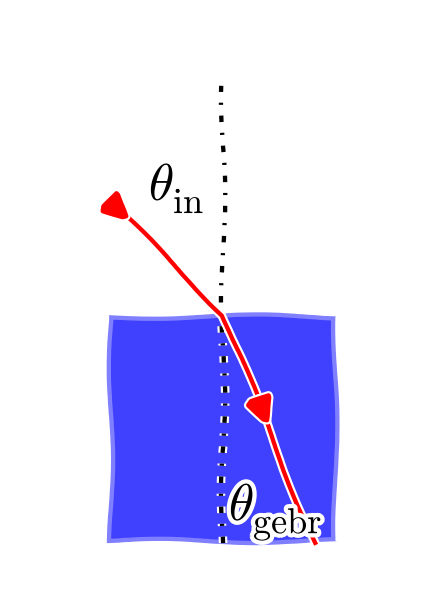
\includegraphics[scale=0.15, angle=90]{brechung}
  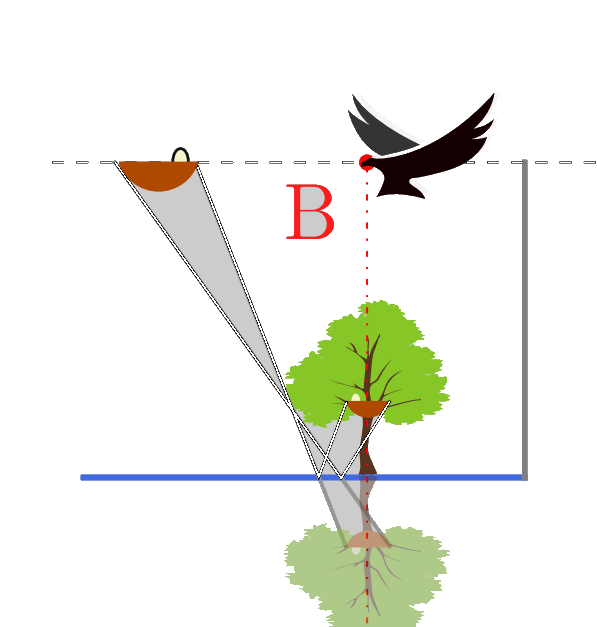
\includegraphics[scale=0.15, angle=0]{voge}
  $$n_1\sin \theta _{in} = n_2\sin \theta _{gebr.}$$

  \subsection{Fermatsches Prinzip}
  Aus der Menge aller möglichen Pfade, die das Licht von einem Punkt zum anderen nehmen
  könnte, nimmt es tatsächlich denjenigen Pfad, entlang dem es die kurzeste Zeit benötigt.

  \subsection{Ausbreitungsgeschwindigkeit in einem Medium}
  $$c_M = \frac{c}{n_M(\lambda)}$$

  \subsection{Brechung für sphärische Oberflächen}
  $$\frac{n}{s}+\frac{n'}{s'}= \frac{n'-n}{R}$$
  $n$: Brechungsindex

  \subsection{Fokale Längen (Brennweiten) an spärischen Oberflächen}
  $$f'=\frac{n'R}{n'-n}; f = \frac{nR}{n'-n}$$
  \subsection{Brechungsgesetz für sphärische Oberflächen}
  $\frac{n}{s}+\frac{n'}{s'}=\frac{n}{f}= \frac{n'}{f'}$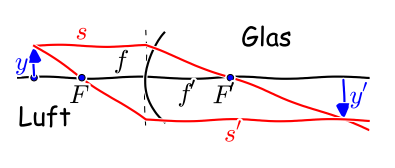
\includegraphics[scale=0.3, angle=0]{konstruktion}
  $$\frac{y'}{y}=\frac{f}{s-f}$$

  \subsection{Linsengleichung}
  $$\frac{1}{s}+\frac{1}{s'} = \frac{1}{f}$$

  \subsection{Linsensysteme}
  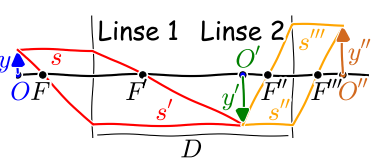
\includegraphics[scale=0.3, angle=0]{lupe}

  \subsection{Elektromagnetismus}
  $$\vec{F}_C(\vec{r})= q\vec{E}$$
  $$\vec{E} = \vec{E}_0\cos [2\pi (x/\lambda-ft)];x \rightarrow r \mathrm{\ für \ Kugelwelle}$$
  $$I_{Intensit.} = \frac{1}{2}c\epsilon _0 E_0^2, [I]=\frac{J}{sm^2}$$
  \textbf{Divergenz eines Lichtstrahls}:
  $$\tan(\mu)=\sin(\mu)=\mu=\frac{\lambda}{D}$$
  \textbf{Bose–Einstein Verteilung}: mittlere Zahl von Photonen in einer Eigenmode der Frequenz fk, die im
  thermischen Gleichgewicht mit den Behälterwänden der Temperatur T ist.
  $$n_K=\frac{1}{exp(\frac{hf_k}{k_BT})-1}$$
  \textbf{Planksches Strahlungsgesetz}: Energie pro Volumen des elektromagnetischen Feldes im Kasten der Temperatur
  $T$, im Wellenlängenbereich $[\lambda, \lambda + d\lambda]$.
  $$U=\frac{8\pi h c}{\lambda ^5}\frac{1}{exp(hc/\lambda k_BT)-1}$$
  \textbf{Wiensches Verschiebungsgesetz}: Wellenlänge bei grösster Leistung/Energiedichte
  $$\lambda = 0.201\frac{hc}{k_BT}=2.898*10^{-3}*1/T$$
  \textbf{Stefan-Boltzmann-Gesetz (Schwarze Körper)}:
  $$P=\sigma A T^4$$
  $\sigma = \frac{2\pi^5k_B^4}{15h^3c^2}=5.67*10^{-8}\frac{W}{m^2K^4}$$

\end{document}
